% -*- Mode:TeX -*-

%% IMPORTANT: The official thesis specifications are available at:
%%            http://libraries.mit.edu/archives/thesis-specs/
%%
%%            Please verify your thesis' formatting and copyright
%%            assignment before submission.  If you notice any
%%            discrepancies between these templates and the 
%%            MIT Libraries' specs, please let us know
%%            by e-mailing thesis@mit.edu

%% The documentclass options along with the pagestyle can be used to generate
%% a technical report, a draft copy, or a regular thesis.  You may need to
%% re-specify the pagestyle after you \include  cover.tex.  For more
%% information, see the first few lines of mitthesis.cls. 

%\documentclass[12pt,vi,twoside]{mitthesis}
%%
%%  If you want your thesis copyright to you instead of MIT, use the
%%  ``vi'' option, as above.
%%
%\documentclass[12pt,twoside,leftblank]{mitthesis}
%%
%% If you want blank pages before new chapters to be labelled ``This
%% Page Intentionally Left Blank'', use the ``leftblank'' option, as
%% above. 

\documentclass[12pt,twoside]{mitthesis}
\usepackage{lgrind}
%% These have been added at the request of the MIT Libraries, because
%% some PDF conversions mess up the ligatures.  -LB, 1/22/2014
\usepackage{cmap}
\usepackage[T1]{fontenc}
\pagestyle{plain}

%% This bit allows you to either specify only the files which you wish to
%% process, or `all' to process all files which you \include.
%% Krishna Sethuraman (1990).

\usepackage{graphicx}

\begin{document}

%THIS IS THE COVER
% Some departments (e.g. 5) require an additional signature page.  See
% signature.tex for more information and uncomment the following line if
% applicable.
% \include{signature}
\pagestyle{plain}
\tableofcontents
\listoffigures
%\listoftables
\chapter{Introduction}
\section{Introduction}
As mobile technologies advance further connectivity becomes increasingly more important. Latest developments in smart phone industry created an environment where many devices communicate with each other. In this context Bluetooth technology makes it possible to connect together various devices with diverse sizes and complexities. On the other hand, FPGAs power many consumer electronics and industrial applications. \cite{eetimes-fpga} Internet of things has become a growing industry on its own with many practical applications and even FPGAs solely targeting this market are being developed. \cite{eetimes-lattice} Combining the technologies described above gives way to innovative applications and this is the main motivation behind this study.

In light of these developments this thesis explores a proof of concept application which establishes communication between a smart phone and a FPGA based system.

\section{Objective}
Primary objective of this work is to develop an application where an Android App can communicate with a FPGA based system using Bluetooth connection and manipulate data on the FPGA.

\section{Scope}
Requirements for this project are as follows:
\begin{itemize}
	\item Android App should be able to transfer 16 8-bits numbers to FPGA over Bluetooth
	\item Android App should have an user friendly interface
	\item FPGA based system can receive data sent from Android App
	\item FPGA based system can save the data to a memory block which can be accessed by other FPGA modules
	\item Data on memory block can be observed from a display unit
\end{itemize}

\chapter{Preliminaries}

This chapter presents an overview of relevant information on hardware, software and tools used in the implementation of this project.  

\section{Microblaze}
The MicroBlaze embedded processor soft core is a reduced instruction set computer (RISC)
optimized for implementation in Xilinx® Field Programmable Gate Arrays (FPGAs). \cite{mb-reference}


\begin{figure}
	\centering
	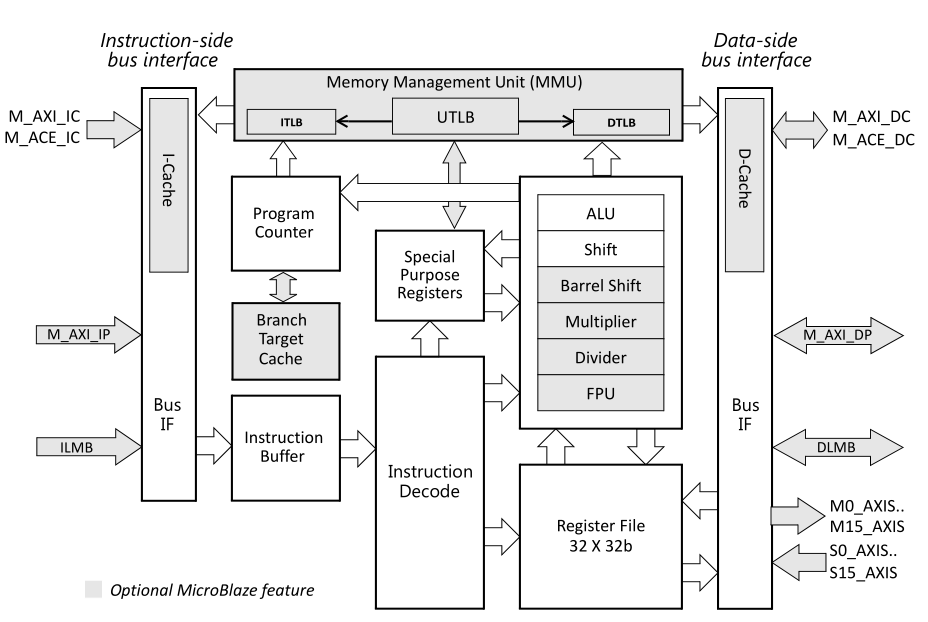
\includegraphics[scale=0.5]{images/microblaze_block_diagram.png}
	\caption{Microblaze block diagram}
\end{figure}


\subsection{Architecture}

The MicroBlaze soft core processor is highly configurable, allowing to select a specific set of features required by design.
The fixed feature set of the processor includes:
\begin{itemize}
	\item Thirty-two 32-bit general purpose registers
	\item 32-bit instruction word with three operands and two addressing modes
	\item Default 32-bit address bus, extensible to 64 bits on the data side
	\item Single issue pipeline
\end{itemize}

In addition to these fixed features, the MicroBlaze processor is parametrized to allow
selective enabling of additional functionality.

All MicroBlaze instructions are 32 bits and are defined as either Type A or Type B. Type A
instructions have up to two source register operands and one destination register operand.
Type B instructions have one source register and a 16-bit immediate operand (which can be
extended to 32 bits by preceding the Type B instruction with an imm instruction). Type B
instructions have a single destination register operand. Instructions are provided in the
following functional categories: arithmetic, logical, branch, load/store, and special.
Table 2-6 lists the MicroBlaze instruction set. 

MicroBlaze has an orthogonal instruction set architecture. It has thirty-two 32-bit general
purpose registers and up to eighteen 32-bit special purpose registers, depending on
configured options.

The thirty-two 32-bit General Purpose Registers are numbered R0 through R31. The register
file is reset on bit stream download (reset value is 0x00000000). Figure 2-2 is a
representation of a General Purpose Register and Table 2-7 provides a description of each
register and the register reset value (if existing).

MicroBlaze supports reset, interrupt, user exception, break, and hardware exceptions.

The relative priority starting with the highest is:
\begin{enumerate}
	\item Reset
	\item Hardware Exception
	\item Non-maskable Break
	\item Break
	\item Interrupt
	\item User Vector (Exception)
\end{enumerate}

\subsection{Signal Interface}

The MicroBlaze core is organized as a Harvard architecture with separate bus interface units
for data and instruction accesses. The following two memory interfaces are supported:
Local Memory Bus (LMB), and the AMBA® AXI4 interface (AXI4) and ACE interface (ACE).
The LMB provides single-cycle access to on-chip dual-port block RAM. The AXI4 interfaces
provide a connection to both on-chip and off-chip peripherals and memory. The ACE
interfaces provide cache coherent connections to memory.
MicroBlaze also supports up to 16 AXI4-Stream interface ports, each with one master and
one slave interface.

MicroBlaze can be configured with the following bus interfaces:
\begin{itemize}
	\item The AMBA AXI4 Interface for peripheral interfaces, and the AMBA AXI4 or AXI
	Coherency Extension (ACE) Interface for cache interfaces
	\item LMB provides a simple synchronous protocol for efficient block RAM transfers
	\item AXI4-Stream provides a fast non-arbitrated streaming communication mechanism
	\item Debug interface for use with the Microprocessor Debug Module (MDM) core
	\item Trace interface for performance analysis
\end{itemize}


\subsection{Xilinx EDK}

The Embedded Development Kit (EDK) is an integrated development environment for designing embedded processing systems. This pre-configured kit includes Xilinx Platform Studio and the Software Development kit, as well as all the documentation and IP that you require for designing Xilinx Platform FPGAs with embedded PowerPC hard processor cores and/or MicroBlaze soft processor cores.
The Embedded Development Kit Provides:

Xilinx Platform Studio (XPS) Tool Suite - Including: Graphical IDE and command line support for developing hardware platforms for embedded applications.  The Base System Builder wizard enables creation of a working embedded system within minutes.  XPS also includes other intelligent design wizards to quickly configure the embedded system architecture, buses and peripherals.

Software Development Kit (SDK) for MicroBlaze and PowerPC - Including: GNU C/C++ compiler and debugger; Xilinx Microprocessor Debug (XMD) target server; Data2MEM utility for bitstream loading and updating.  SDK is the recommended software-centric design environment based on the Eclipse IDE.

Real-Time Operating System and Embedded OS Support - Provides design support and board support package (BSP) generation for numerous third party suppliers in the Xilinx ecosystem, including vendors such as Wind River, Green Hills, Mentor, LynuxWorks and other embedded industry leaders.

Processing IP and MicroBlaze Soft Processor Core -Pre-verified IP catalog, including a wide variety of processing peripheral cores for customizing your embedded systems as well as the flexible MicroBlaze 32-bit soft processing core. The MicroBlaze processor offers memory management and FPU configuration options enabling commercial grade RTOS support, unique for a soft processor. \cite{xilinx-xps-edk}

\section{Pmod CLS}
The Digilent PmodCLS is a 16x2 character LCD module driven by an Atmel ATmega48 microcontroller.

\begin{figure}
	\centering
	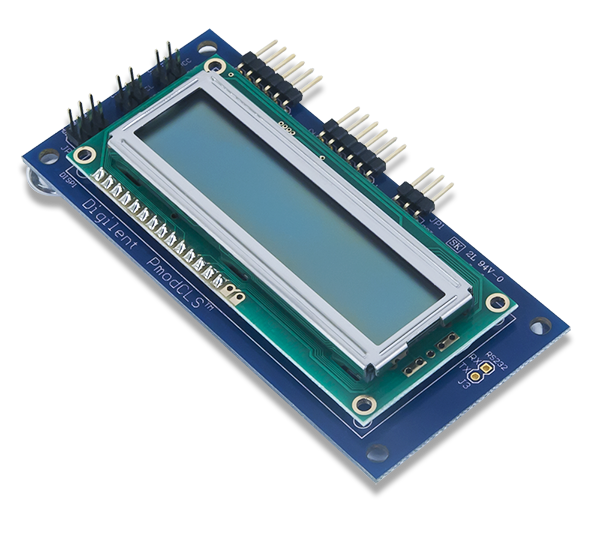
\includegraphics{images/pmodcls-product.png}
	\caption{Pmod CLS LCD Module}
\end{figure}

\begin{figure}[h]
	\centering
	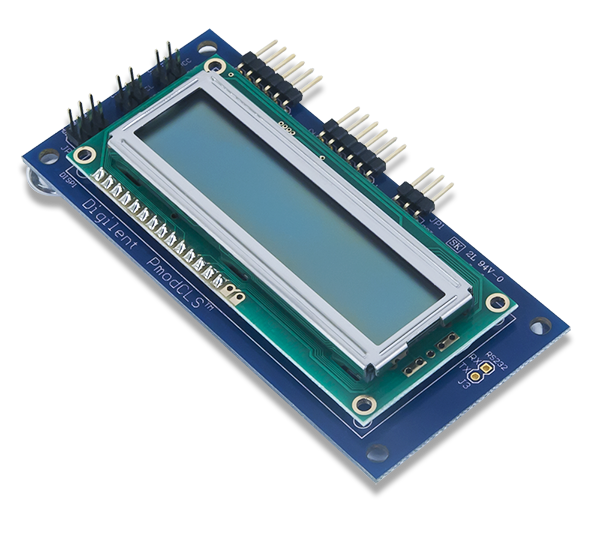
\includegraphics[width=0.7\linewidth]{images/pmodcls-product}
	\caption[Pmod CLS LCD Module]{}
	\caption{}
	\label{fig:pmodcls-product}
\end{figure}

The PmodCLS module can be used to display important information during program development or as a user
interface after the project has been completed. The module is ideally suited for microcontroller boards but can
also be used in projects using a FPGA board.
The module is capable of executing a variety of instructions such as erasing specific characters, setting different
display modes, scrolling, and displaying user-defined characters. These instructions are specified using escape
sequences to send commands to the board’s embedded Atmel ATmega48 microcontroller. The display on the
module is driven by this AVR and controls all of the features of the board.

The PmodCLS can communicate with the host board through the SPI, I 2 C, and UART ports.Through these protocol standards, users are able to set the cursor location and send other instructions by sending
escape sequences. And escape sequence is specified by first sending the escape character (0x1B) followed by a left square bracket '[' (0x5B), and then one or more numeric parameters followed by the command character for the specific command.

\section{HC-06 Bluetooth Module}

HC-06 module is a low-cost Bluetooth module which can be used by any UART implementation. This module works slave mode only and supports AT commands. By default the baud rate of device is set to 9600, however it can be set to a different rate by using AT commands.

\begin{figure}
	\centering
	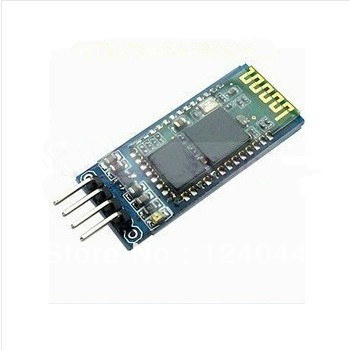
\includegraphics[scale= 0.6]{images/hc-06.jpg}
	\caption{HC-06 Bluetooth Module}
\end{figure}

The module has four external pins; 
VCC : Power Supply
GND : Ground
TXD : Transmitter
RXD : Receiver   

The pin which TXD module connects to must be set to PULLUP mode to ensure reliable data transfer. 


\section{Digilent Nexys 3 FPGA Board}

The Nexys 3 is a complete, ready-to-use digital circuit development platform based on the Xilinx Spartan-6 LX16 FPGA. The Spartan-6 is optimized for high performance logic, and offers more than 50\% higher capacity, higher performance, and more resources as compared to the Nexys 2's Spartan-3 500E FPGA.

\begin{figure}
	\centering
	\includegraphics[scale=0.2]{images/nexys-3.png}
	\caption{Nexys 3 Spartan 6 Development Board}
\end{figure}

Features include:

\begin{itemize}
\item Xilinx Spartan-6 LX16 FPGA in a 324-pin BGA package
\item 16Mbyte Cellular RAM (x16)
\item 16Mbytes SPI (quad mode) PCM non-volatile memory
\item 16Mbytes parallel PCM non-volatile memory
\item 10/100 Ethernet PHY
\item USB-UART and USB-HID port (for mouse/keyboard)
\item 8-bit VGA port
\item 100MHz CMOS oscillator
\item 72 I/Os routed to expansion connectors
\item GPIO includes 8 LEDs, 5 buttons,8 slide switches and 4-digit seven-segment display
\end{itemize}

\begin{figure}
	\centering
	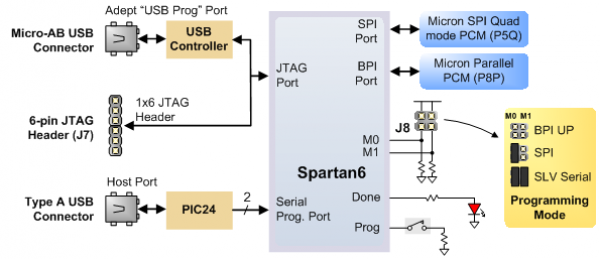
\includegraphics[scale=0.7]{images/nexys-3-config.png}
	\caption{Nexys 3 Configuration }
\end{figure}

\section{Software}

Two different software developed for the complete project. One is written in C and compiled using Microblaze Toolchain provided by Xilinx EDK \cite{xilinx-xps-edk}. The other written in Java and compiled with Android SDK provided by Android Studio \cite{android-studio}. 

\section{Android}
Android is an open source, Linux-based software stack created for a wide array of devices and form factors.

\begin{figure}
	\centering
	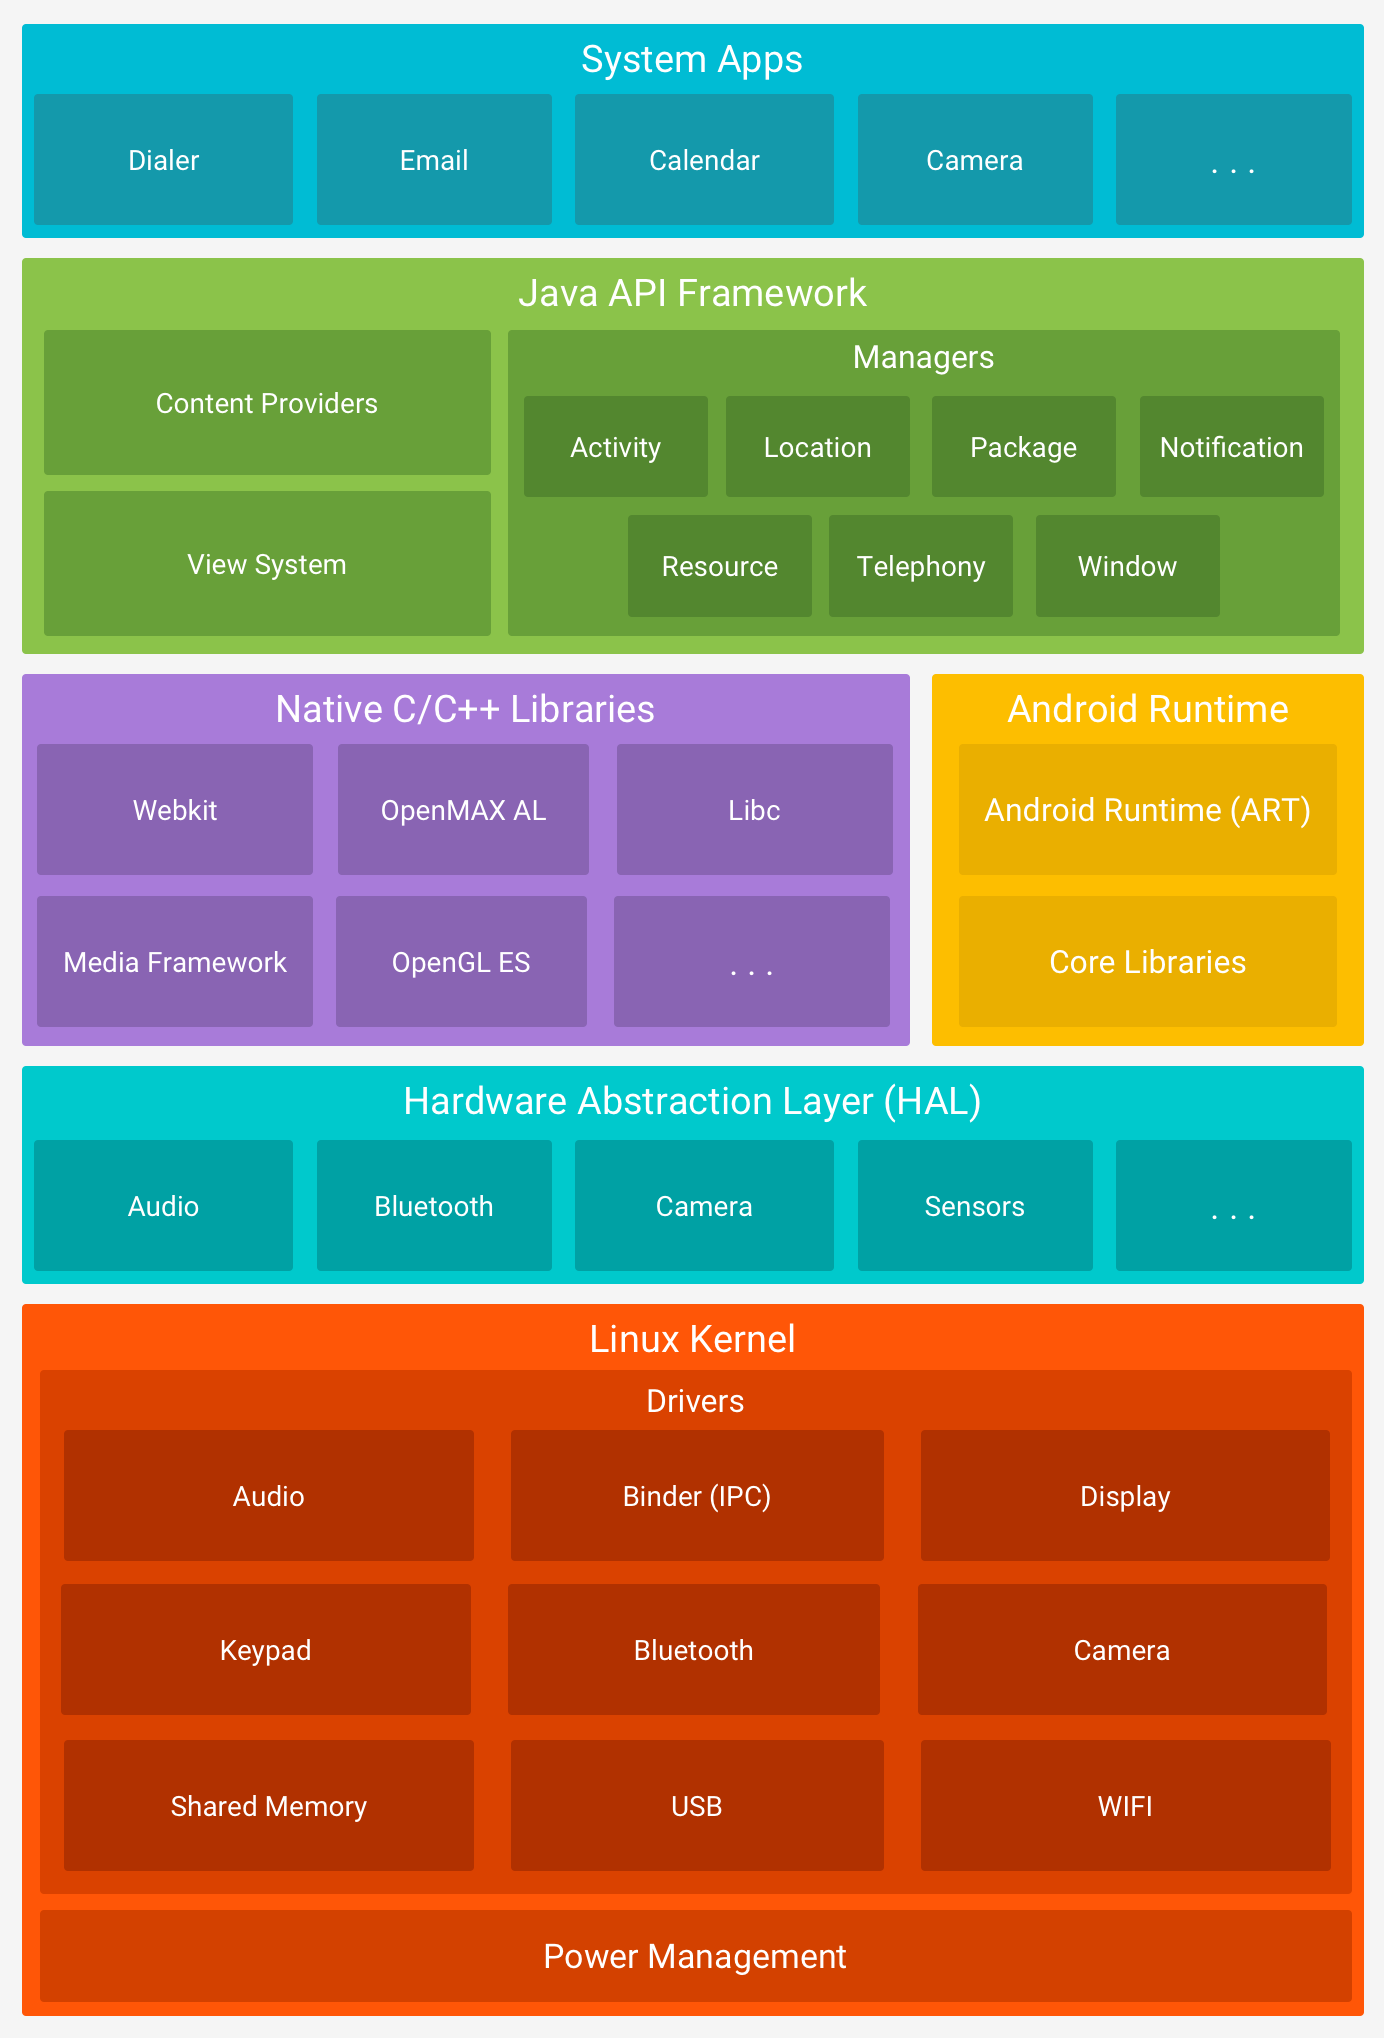
\includegraphics[scale=0.1]{images/android-stack.png}
	\caption{The Android software stack}
\end{figure}

Android provides a rich application framework that allows to build innovative apps and games for mobile devices in a Java language environment. Android apps are built as a combination of distinct components that can be invoked individually. For instance, an individual activity provides a single screen for a user interface, and a service independently performs work in the background.

Android apps are written in the Java programming language. The Android SDK tools compile code along with any data and resource files into an APK, an Android package, which is an archive file with an .apk suffix. One APK file contains all the contents of an Android app and is the file that Android-powered devices use to install the app.

App components are the essential building blocks of an Android app. Each component is an entry point through which the system or a user can enter your app. Some components depend on others.

There are four different types of app components:
\begin{itemize}
\item Activities
\item Services
\item Content providers
\item Broadcast receivers
\end{itemize}

Each type serves a distinct purpose and has a distinct lifecycle that defines how the component is created and destroyed. Three of the four component types—activities, services, and broadcast receivers—are activated by an asynchronous message called an intent. Intents bind individual components to each other at runtime. 

An Android app is composed of more than just code, it requires resources that are separate from the source code, such as images, audio files, and anything relating to the visual presentation of the app. For example; animations, menus, styles, colors, and the layout of activity user interfaces can be defined with XML files. Using app resources makes it easy to update various characteristics of an app without modifying code. Providing sets of alternative resources enables to optimize an app for a variety of device configurations, such as different languages and screen sizes. \cite{android-developer}


\chapter{Processor Design}
Lorem ipsum dolor sit amet, consectetur adipiscing elit. Curabitur quis nisl nibh. Vivamus viverra eleifend metus et tincidunt. Mauris quis ullamcorper ante. Nulla quis vehicula nisi. Aenean in vehicula turpis. Curabitur gravida, arcu a rutrum commodo, lectus leo vulputate dui, a cursus justo quam eget ipsum. Praesent blandit metus vitae lacus vehicula porttitor.
\section{Overview}
Pellentesque hendrerit leo tortor. Donec pretium eleifend mi. Vivamus dapibus eget massa vel ultrices. In hac habitasse platea dictumst. In nec risus sit amet lectus sagittis viverra at sit amet nulla. Cras sed massa auctor, efficitur mauris ac, elementum elit. Nulla facilisi. Nunc molestie pretium ligula, at pretium nunc laoreet at. Proin id auctor sem. Donec eu velit posuere, pharetra diam nec, auctor dui. Donec ac egestas enim. Nullam vel arcu vehicula, suscipit orci id, accumsan nunc. Maecenas accumsan, orci a venenatis fermentum, dui urna aliquam dolor, in placerat mauris est at sapien. Donec gravida malesuada turpis ac pharetra.
\subsection{Processor Overview}
Quisque finibus elit dui, egestas elementum mauris suscipit vitae. Proin et hendrerit tortor, id iaculis orci. Sed vehicula sed magna id sodales. Maecenas ultricies risus nec ornare dignissim. In vitae finibus orci. Nam vel aliquam urna. Sed iaculis dictum neque. Pellentesque a convallis lacus. Nullam auctor vel nulla a convallis. Ut nec suscipit arcu.
\section{Processor Design}
Donec suscipit est vel pretium interdum. Morbi malesuada risus sit amet neque pharetra sodales sit amet et lacus. Vestibulum vel euismod tellus. Nam in consequat nunc. Suspendisse potenti. Etiam commodo porta suscipit. Proin finibus sed enim eget ultrices. Mauris eu nunc enim. Aenean et felis id lorem viverra euismod. Aliquam vehicula sodales est sed iaculis. Morbi mattis vehicula massa sit amet congue.

Nullam tempor, metus ut consectetur volutpat, diam arcu viverra ligula, fermentum porttitor dui ligula non nisi. Etiam dui risus, malesuada dapibus felis vitae, pharetra vulputate purus. Vivamus quis blandit ligula, tincidunt bibendum turpis. Sed ac est justo. Curabitur at magna a ligula porttitor gravida. Nullam euismod ipsum faucibus, luctus purus sit amet, accumsan est. Morbi nec tortor non velit gravida bibendum eget in ex. Cras tristique posuere lacus, a blandit ipsum pulvinar sed. Vivamus nec velit aliquet, rutrum diam ac, egestas massa. 



%\appendix
%\include{appa}
%\include{appb}
\bibliographystyle{plain}
\bibliography{biblio}
\end{document}

